\begin{CJK*}{UTF8}{zhhei}
    \zihao{5}
    \vskip 1mm
    \section{实验}
\end{CJK*}


\begin{CJK*}{UTF8}{zhhei}
    \subsection{实验设置}
\end{CJK*}

\begin{CJK*}{UTF8}{zhhei}
    \subsubsection{数据集}
\end{CJK*}
本文在Pascal VOC 2012\cite{18everingham2010pascal}数据集上评估所提方法。Pascal VOC 2012包含20个前景类别和1个背景类别。它有三个子集:训练集(train)、验证集(val)和测试集(test),分别包含1464、1449 和 1456张图片。按照先前方法\cite{06wang2020self,12xu2022multi,13ru2022learning,03ru2023token}的常用做法,本文进一步利用SBD数据集将VOC训练集图片数量扩充至10582。在训练过程中,本文严格只使用图像级分类标签用于监督模型训练。

\begin{CJK*}{UTF8}{zhhei}
    \subsubsection{评估指标}
\end{CJK*}
与先前方法一样,本文使用平均交并比(mean Intersection over Union,mIoU),作为CAM质量、伪标签质量以及语义分割模型性能的评估指标。本文方法在Pascal VOC测试集上的评估结果由官方在线评估服务器给出。

\begin{CJK*}{UTF8}{zhhei}
    \subsubsection{实现细节}
\end{CJK*}

\begin{figure*}[t]
    \centerline{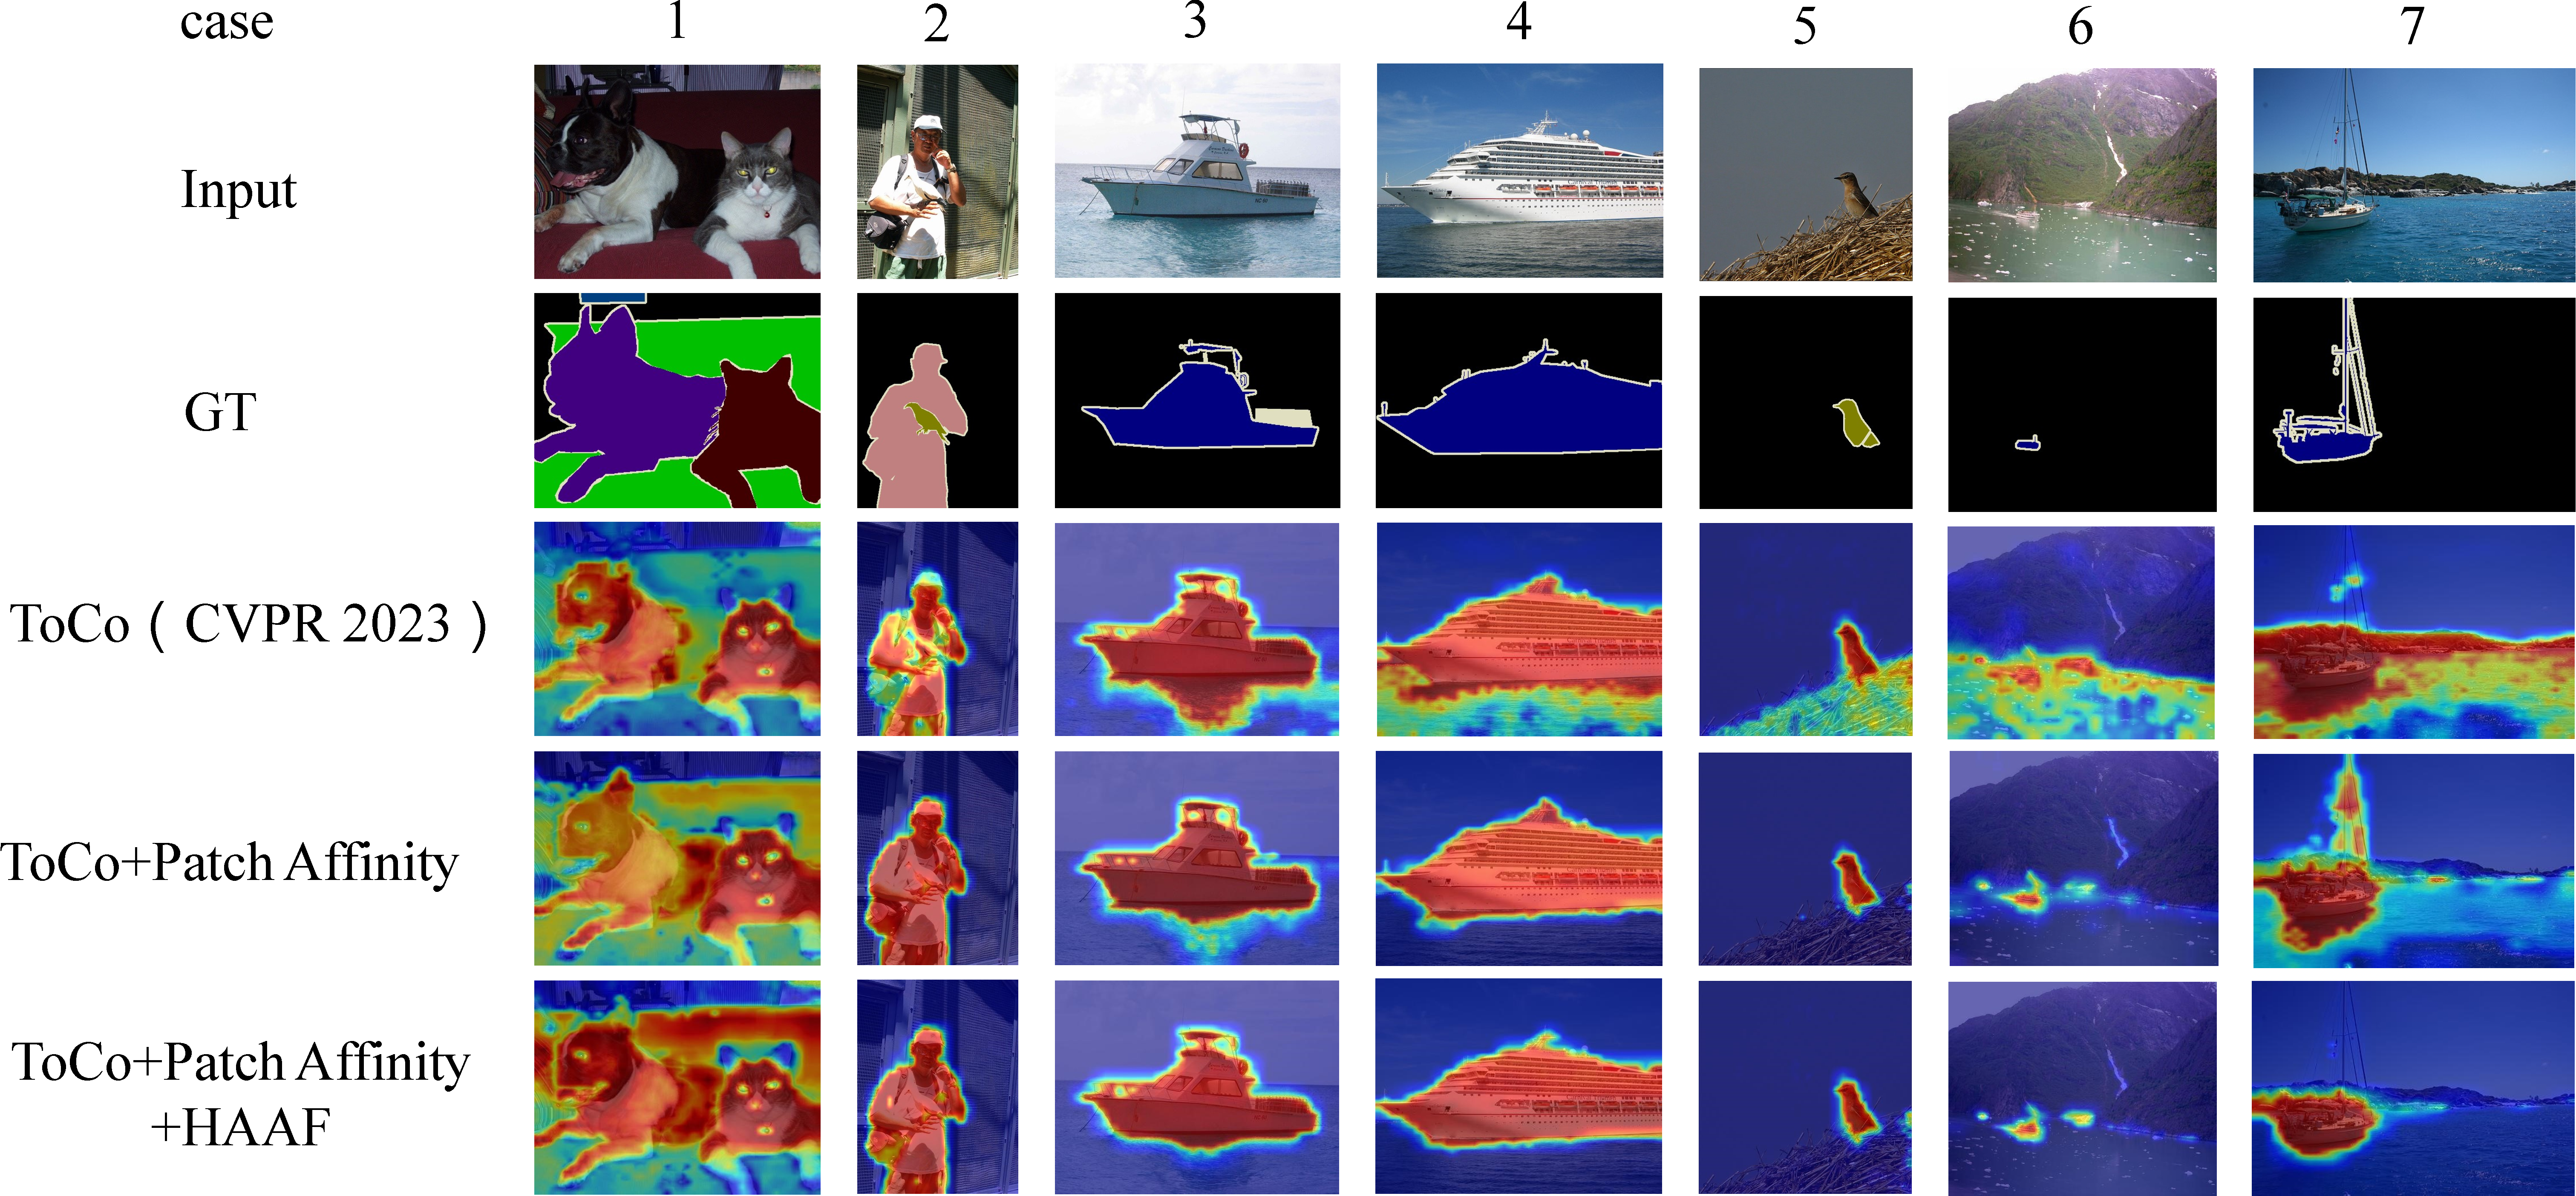
\includegraphics[width=6in]{fig/fig5.pdf}}
    \begin{CJK*}{UTF8}{fs}
        \caption{生成CAM可视化结果,从上到下依次为输入图片(input),真值标签(GT),ToCo生成CAM,SS-EPA生成CAM(不使用HAAF),SS-EPA生成CAM(使用HAAF)。红框部分为显著提升区域。}\label{fig5}
    \end{CJK*}
\end{figure*}

本文利用在 ImageNet 数据集\cite{19deng2009imagenet}上预训练的ViT-B(vit\_base\_patch16\_224)\cite{02dosovitskiy2020image}作为 backbone,它有$12$层 Transformer 编码层,$12$个注意力头,嵌入维度为$768$。卷积解码器使用 LargeFOV \cite{20chen2017deeplab},它由两个膨胀系数为$5$的$3\times 3$卷积和一个$1\times 1$卷积预测层构成。

输入图片被随机裁剪为$448\times 448$的大小。模型共训练$20000$个迭代,batch-size设置为$4$,模型优化器采用AdamW\cite{21loshchilov2017decoupled},学习率在前$1500$个迭代中逐渐提升到$6\times 10^{-5}$,并在后续根据多项式调度器衰减。公式\ref{equation_8}中的权重因子$\lambda_i,i=1,2,…,5$在前$2000$个迭代分别设置为($0, 1.0, 0.2, 0.5, 0$),$2000$个迭代后分别设置为($0.1, 1.0, 0.2, 0.5, 0.05$)。

\vspace{2mm}

\begin{CJK*}{UTF8}{zhhei}
    \subsection{实验结果}
\end{CJK*}
\begin{CJK*}{UTF8}{zhhei}
    \subsubsection{CAM与伪标签}
\end{CJK*}

\begin{table}[t]
    \setlength{\tabcolsep}{4mm}
    \tiny
    \centering
    \caption{伪标签生成定量评估(MS:Multi Scale,CRF:dense CRF)(单位mIoU\%)}\label{table1}
    \begin{tabular}{lccc}
        \toprule
        Method & Backbone & train & val \\
        \midrule
        \textbf{\textit{Multi-Stage WSSS Methods}}& & &\\
        ViT-PCM\cite{23rossetti2022max}	& ViT-B & 67.7 & 66.0\\
        MCTformer\cite{12xu2022multi} & Deit-S & 69.1 & -\\
        LPCAM\cite{24chen2023extracting} & Deit-S & - & 70.8\\
        SFC\cite{26zhao2024sfc} & ResNet101 & 73.7 & -\\
        POLE\cite{25murugesan2024prompting} & ResNet50 & 74.2 & -\\
        \cmidrule[0.4pt](lr){1-4}
        \textbf{\textit{Single-Stage WSSS Methods}}& & &\\
        RRM\cite{17zhang2020reliability} & ResNet38 & - & 65.4\\
        1Stage\cite{27araslanov2020single} & ResNet38 & 66.9 & 65.3\\
        SLRNet\cite{28pan2022learning} & ResNet38 & 67.1 & 66.2\\
        AFA\cite{13ru2022learning} & MiT-B1 & 68.7 & 66.5\\
        MCC\cite{29wu2024masked} & Deit-B & 75.1 & 72.2\\
        ToCo\cite{03ru2023token} & ViT-B & 74.5 & 72.2\\
        ToCo+MS+CRF\cite{03ru2023token} & ViT-B & 77.3 & 74.6\\
        \textbf{SSEPA} & \textbf{ViT-B} & \textbf{77.1} & \textbf{74.2}\\
        \bottomrule
    \end{tabular}
\end{table}

图\ref{fig5}呈现了SS-EPA生成CAM的可视化结果,并与基线模型ToCo相比较。可以看出,SS-EPA在不使用HAAF的情况下,生成的CAM比ToCo更少,说明利用原始补丁语义亲和力优化CAM,可以显著减少初始CAM中的噪声,纠正错误激活的背景区域,使CAM更加精准和细化。在使用HAAF后,SS-EPA可能够发现一些未被初始CAM激活的前景区域(如图\ref{fig5}中case~1与case~2),并生成错误更少的CAM(如图\ref{fig5}中case~3至case~7),这说明了本文提出的HAAF可以进一步优化补丁语义亲和力,从而生成更优质的CAM。

% \begin{figure*}[htbp]
%     \centerline{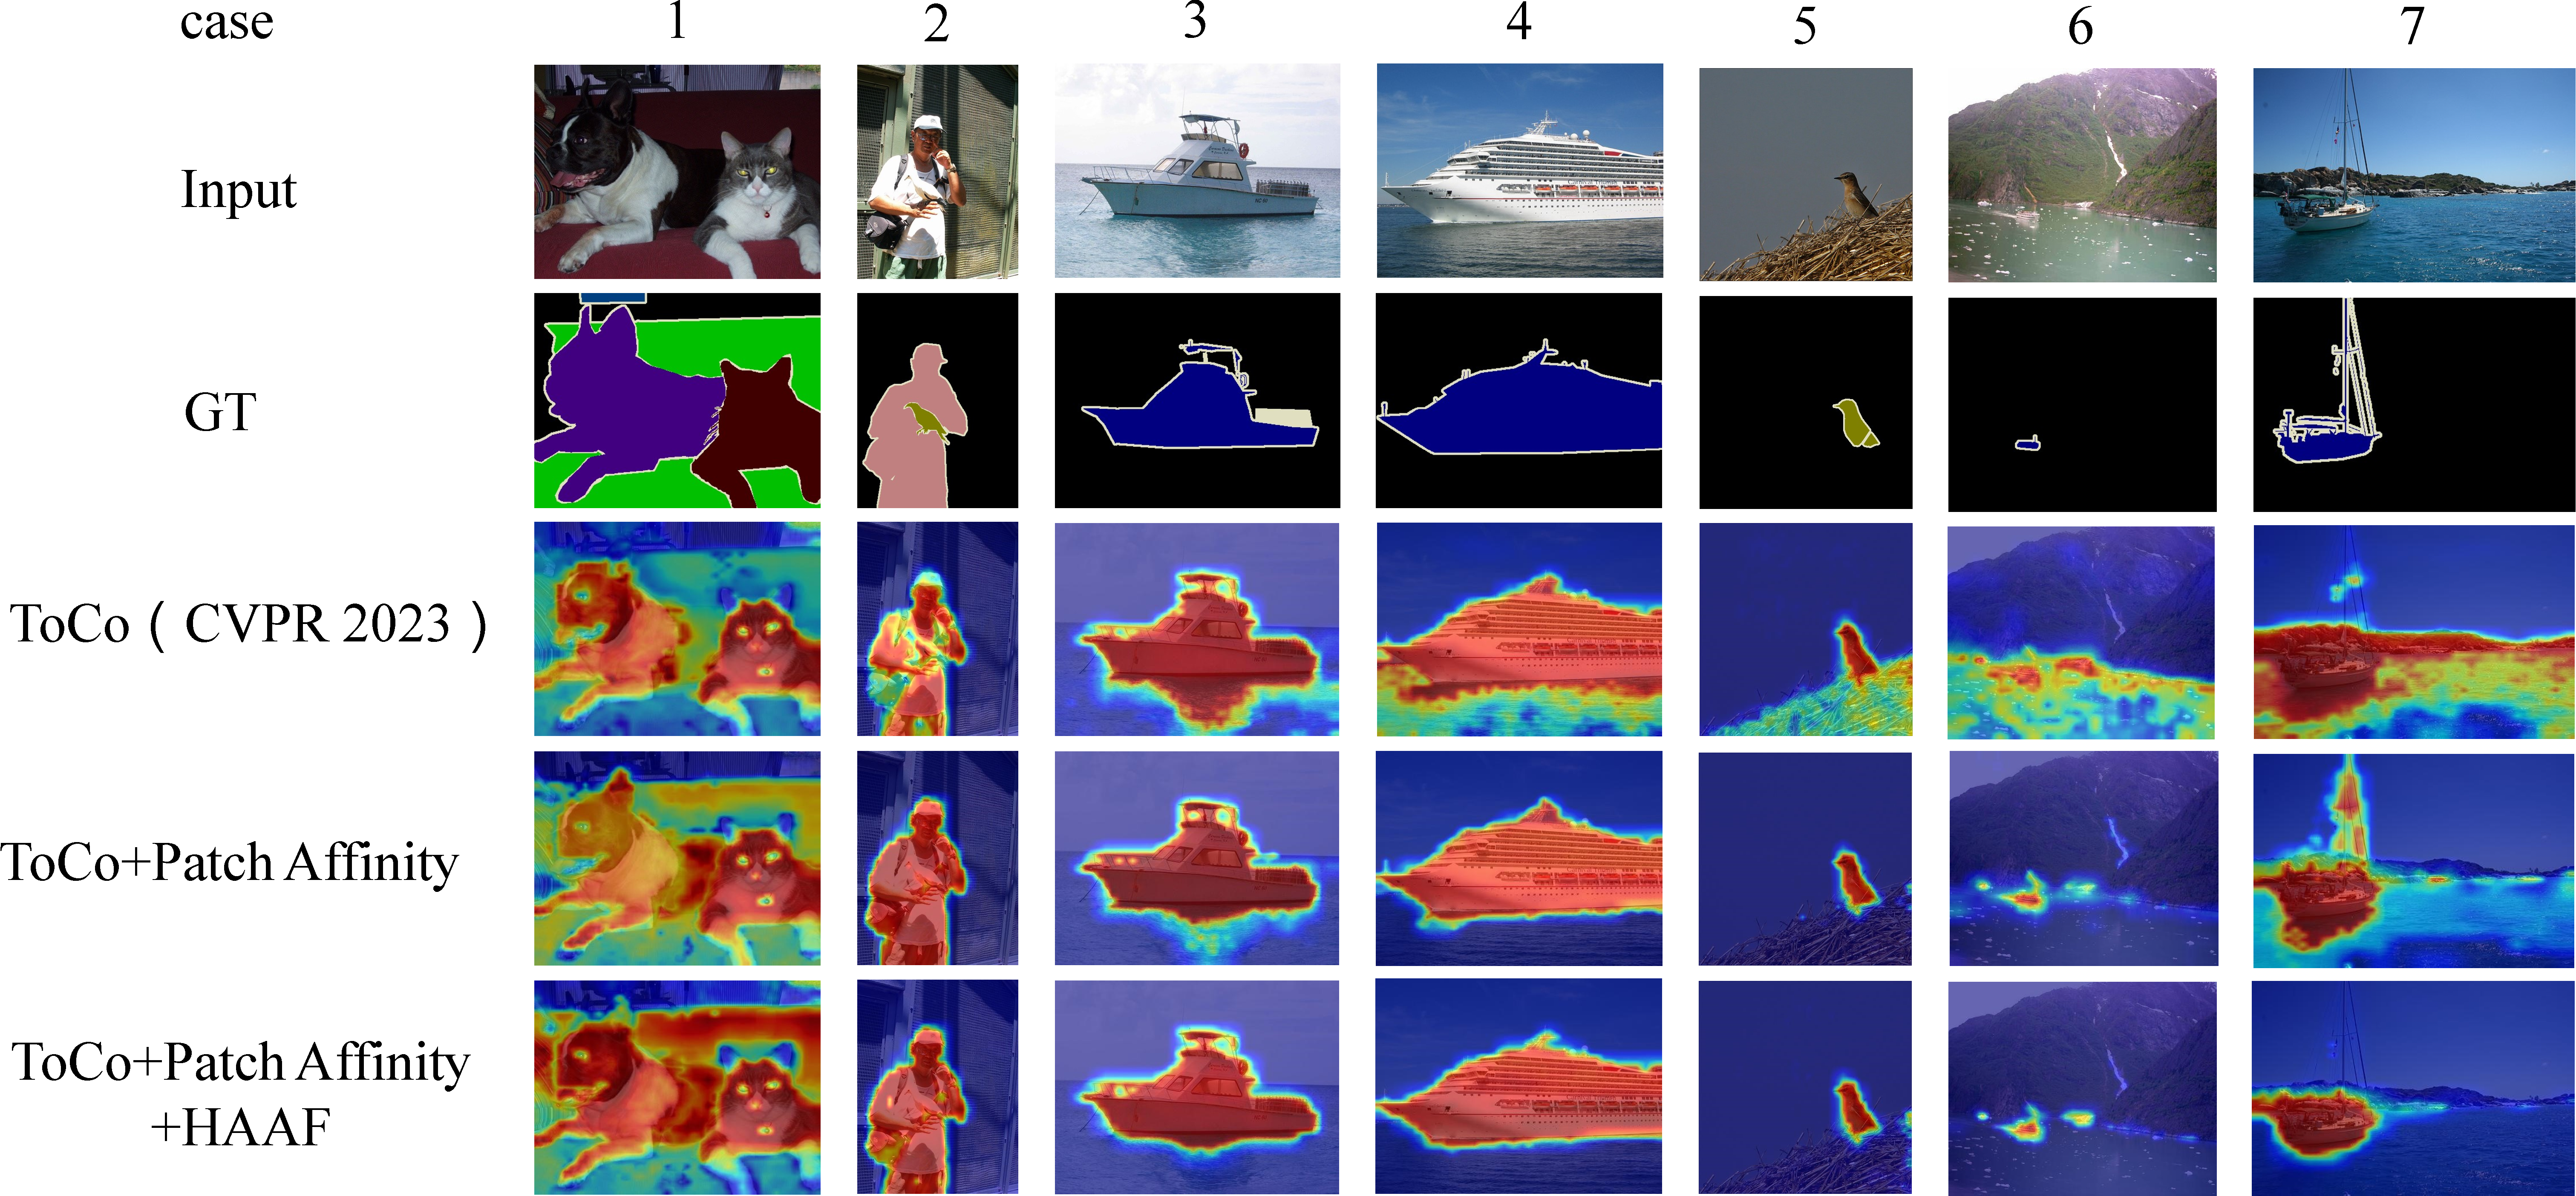
\includegraphics[width=6in]{fig/fig5.pdf}}
%     \begin{CJK*}{UTF8}{fs}
%         \caption{生成CAM可视化结果,从上到下依次为输入图片(input),真值标签(GT),ToCo生成CAM,SS-EPA生成CAM(不使用HAAF),SS-EPA生成CAM(使用HAAF)。红框部分为显著提升区域。}\label{fig5}
%     \end{CJK*}
% \end{figure*}

表\ref{table1}呈现了利用 CAM 生成伪标签的定量评估结果,在 VOC 训练集和验证集上进行评估,并与一些先进的 WSSS 方法进行比较。结果表明,本文提出的 SS-EPA 比现有的单阶段 WSSS 方法更好,且达到了与一些多阶段 WSSS 方法相当的性能。与基线方法 ToCo 相比较,无论是否使用 MS(Multi Scale) 和 CRF(DenseCRF) , SS-EPA 的性能都要优于 ToCo 。

% \begin{table}[t]
%     \setlength{\tabcolsep}{4mm}
%     \tiny
%     \centering
%     \caption{伪标签生成定量评估(MS:Multi Scale,CRF:dense CRF)(单位mIoU\%)}\label{table1}
%     \begin{tabular}{lccc}
%         \toprule
%         Method & Backbone & train & val \\
%         \midrule
%         \textbf{\textit{Multi-Stage WSSS Methods}}& & &\\
%         ViT-PCM\cite{23rossetti2022max}	& ViT-B & 67.7 & 66.0\\
%         MCTformer\cite{12xu2022multi} & Deit-S & 69.1 & -\\
%         LPCAM\cite{24chen2023extracting} & Deit-S & - & 70.8\\
%         SFC\cite{26zhao2024sfc} & ResNet101 & 73.7 & -\\
%         POLE\cite{25murugesan2024prompting} & ResNet50 & 74.2 & -\\
%         \cmidrule[0.4pt](lr){1-4}
%         \textbf{\textit{Single-Stage WSSS Methods}}& & &\\
%         RRM\cite{17zhang2020reliability} & ResNet38 & - & 65.4\\
%         1Stage\cite{27araslanov2020single} & ResNet38 & 66.9 & 65.3\\
%         SLRNet\cite{28pan2022learning} & ResNet38 & 67.1 & 66.2\\
%         AFA\cite{13ru2022learning} & MiT-B1 & 68.7 & 66.5\\
%         MCC\cite{29wu2024masked} & Deit-B & 75.1 & 72.2\\
%         ToCo\cite{03ru2023token} & ViT-B & 74.5 & 72.2\\
%         ToCo+MS+CRF\cite{03ru2023token} & ViT-B & 77.3 & 74.6\\
%         \textbf{SSEPA} & \textbf{ViT-B} & \textbf{77.1} & \textbf{74.2}\\
%         \bottomrule
%     \end{tabular}
% \end{table}
\begin{figure*}[htbp]
    \centerline{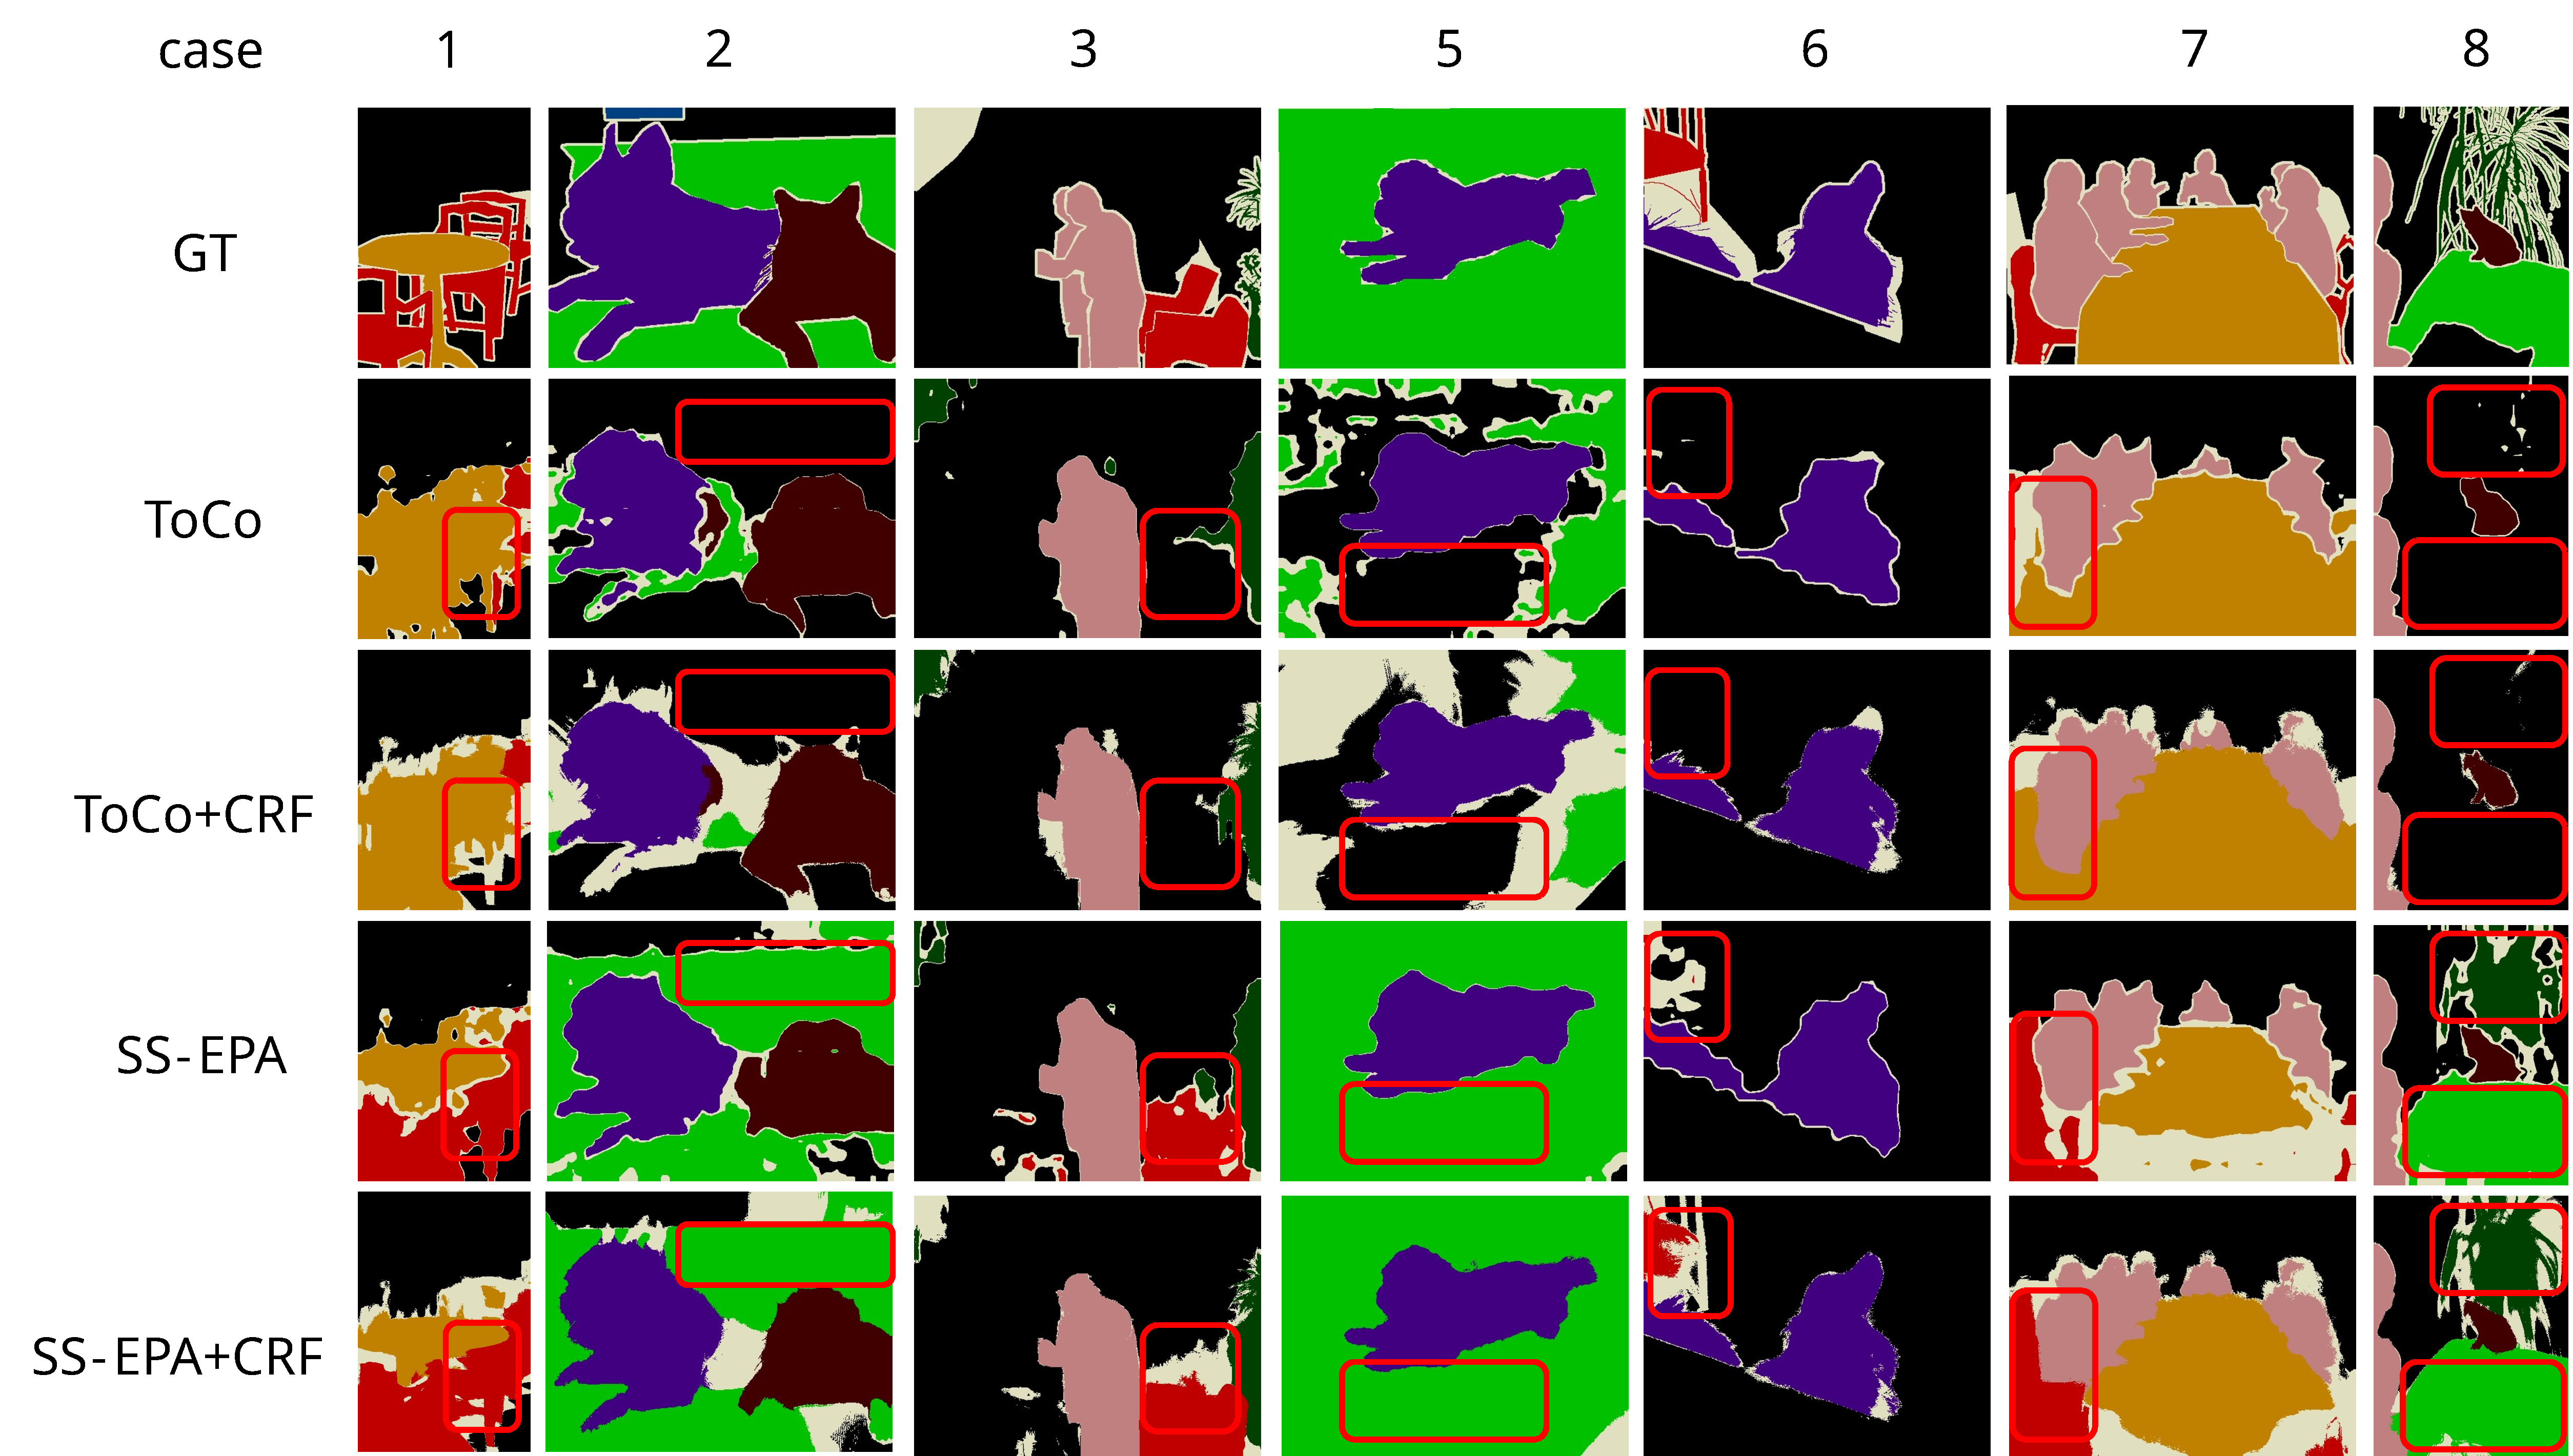
\includegraphics[width=6in]{fig/fig6.pdf}}
    \begin{CJK*}{UTF8}{fs}
        \caption{生成伪标签的可视化结果,从上到下依次为分割真值标签(GT),ToCo分割结果(不加CRF),ToCo分割结果(加CRF),SS-EPA分割结果(不加CRF),SS-EPA分割结果(加CRF)。红框部分为显著提升区域。}\label{fig6}
    \end{CJK*}
\end{figure*}

\begin{table}[htbp]
    
    \normalsize
    \setlength{\tabcolsep}{4mm}
    \centering
    \caption{分割结果定量评估(单位mIoU\%)}\label{table2}
    \tiny
    \begin{tabular}{lccc}
        \toprule
        Method & Backbone & train & val \\
        \midrule
        \textbf{\textit{Multi-Stage WSSS Methods}}& & &\\
        ReCAM\cite{33chen2022class} & ResNet101 & 68.5 & 68.4\\
        ViT-PCM\cite{23rossetti2022max }& ResNet101 & 70.3 & 70.9\\
        CLIMS\cite{08xie2022clims} & ResNet101 & 70.4 & 70.0\\
        AMN\cite{34lee2022threshold} & ResNet101 & 70.7 & 70.6\\
        EDAM\cite{30wu2021embedded} & ResNet101 & 70.9 & 70.6 \\
        SFC\cite{26zhao2024sfc} & ResNet101 & 71.2 & 72.5 \\
        POLE\cite{25murugesan2024prompting} & ResNet50 & 71.5 & 71.4 \\
        MCTformer\cite{12xu2022multi} & Deit-S & 71.9 & 71.6 \\
        L2G\cite{31jiang2022l2g} & ResNet101 & 72.1 & 71.7 \\
        BECO\cite{35rong2023boundary} & ResNet101 & 72.1 & 71.8 \\
        RCA\cite{32zhou2022regional} & ResNet38 & 72.2 & 72.8 \\
        LPCAM\cite{24chen2023extracting} & Deit-S & 72.6 & 72.4 \\
        OCR\cite{36cheng2023out} & ResNet38 & 72.7 & 72.0 \\
        \cmidrule[0.4pt](lr){1-4}
        \textbf{\textit{Single-Stage WSSS Methods}}& & &\\
        RRM\cite{27araslanov2020single} & ResNet38 & 62.6 & 62.9 \\
        1Stage\cite{27araslanov2020single} & ResNet38 & 62.7 & 64.3 \\
        AFA\cite{13ru2022learning} & MiT-B1 & 66.0 & 66.3 \\
        SLRNet\cite{28pan2022learning} & ResNet38 & 67.2 & 67.6 \\
        MCC\cite{29wu2024masked} & Deit-B & 70.3 & 71.2 \\
        ToCo\cite{03ru2023token} & ViT-B & 71.1 & 72.2 \\
        \textbf{SSEPA} & \textbf{ViT-B} & \textbf{72.4} & \textbf{73.2}\\
        \bottomrule
    \end{tabular}
\end{table}

图\ref{fig6}是 SS-EPA 生成伪标签的可视化结果,包括使用 DenseCRF\cite{22chen2014semantic} 后处理前后的结果。可视化结果表明,无论是否使用 CRF,SS-EPA 生成的伪标签在准确度上都高于 ToCo(如图6中 case 1 与case 7),且能识别到一些 ToCo 无法识别到的目标(如图6中 case 2 至 case 6 )。



\begin{CJK*}{UTF8}{zhhei}
    \subsubsection{分割结果}
\end{CJK*}

表\ref{table2}中呈现了在 Pascal VOC 2012 数据集上的定量语义分割结果,比较了本文提出的 SS-EPA 与其它的 WSSS 方法在 mIoU 分数上的表现。 SS-EPA 用ImageNet 预训练的 ViT-B(vit\_base\_patch16\_224) 作为b ackbone,在验证集和测集上分别达到了 72.4\% 和 73.3\% 的mIoU分数,比基线方法 ToCo 提升了 1.3\% 和 1.1\% 的 mIoU 分数。结果表明, SS-EPA 的性能优于现有的利用图像级标签的单阶段 WSSS 方法。此外,SS-EPA 与许多多阶段 WSSS 方法的性能相当,证明了本文所提方法的有效性。


% \begin{table}[htbp]
    
%     \normalsize
%     \setlength{\tabcolsep}{4mm}
%     \centering
%     \caption{分割结果定量评估(单位mIoU\%)}\label{table2}
%     \tiny
%     \begin{tabular}{lccc}
%         \toprule
%         Method & Backbone & train & val \\
%         \midrule
%         \textbf{\textit{Multi-Stage WSSS Methods}}& & &\\
%         ReCAM\cite{33chen2022class} & ResNet101 & 68.5 & 68.4\\
%         ViT-PCM\cite{23rossetti2022max }& ResNet101 & 70.3 & 70.9\\
%         CLIMS\cite{08xie2022clims} & ResNet101 & 70.4 & 70.0\\
%         AMN\cite{34lee2022threshold} & ResNet101 & 70.7 & 70.6\\
%         EDAM\cite{30wu2021embedded} & ResNet101 & 70.9 & 70.6 \\
%         SFC\cite{26zhao2024sfc} & ResNet101 & 71.2 & 72.5 \\
%         POLE\cite{25murugesan2024prompting} & ResNet50 & 71.5 & 71.4 \\
%         MCTformer\cite{12xu2022multi} & Deit-S & 71.9 & 71.6 \\
%         L2G\cite{31jiang2022l2g} & ResNet101 & 72.1 & 71.7 \\
%         BECO\cite{35rong2023boundary} & ResNet101 & 72.1 & 71.8 \\
%         RCA\cite{32zhou2022regional} & ResNet38 & 72.2 & 72.8 \\
%         LPCAM\cite{24chen2023extracting} & Deit-S & 72.6 & 72.4 \\
%         OCR\cite{36cheng2023out} & ResNet38 & 72.7 & 72.0 \\
%         \cmidrule[0.4pt](lr){1-4}
%         \textbf{\textit{Single-Stage WSSS Methods}}& & &\\
%         RRM\cite{27araslanov2020single} & ResNet38 & 62.6 & 62.9 \\
%         1Stage\cite{27araslanov2020single} & ResNet38 & 62.7 & 64.3 \\
%         AFA\cite{13ru2022learning} & MiT-B1 & 66.0 & 66.3 \\
%         SLRNet\cite{28pan2022learning} & ResNet38 & 67.2 & 67.6 \\
%         MCC\cite{29wu2024masked} & Deit-B & 70.3 & 71.2 \\
%         ToCo\cite{03ru2023token} & ViT-B & 71.1 & 72.2 \\
%         \textbf{SSEPA} & \textbf{ViT-B} & \textbf{72.4} & \textbf{73.2}\\
%         \bottomrule
%     \end{tabular}
% \end{table}


图\ref{fig7}展示了SS-EPA、ToCo和真实标签的分割结果。可视化结果表明,本文提出的SS-EPA成功分割了图像中的多个对象,并且与ToCo相比,SS-EPA分类的准确度更高(如图7中Val的case 1、3、4,Test的case 5、7、8),能正确发现一些ToCo中误分类为背景的前景目标(如图7中Val的case 2,Test的case 6),且整体对象边界都更加完整和准确。

\begin{figure*}[htbp]
    \centerline{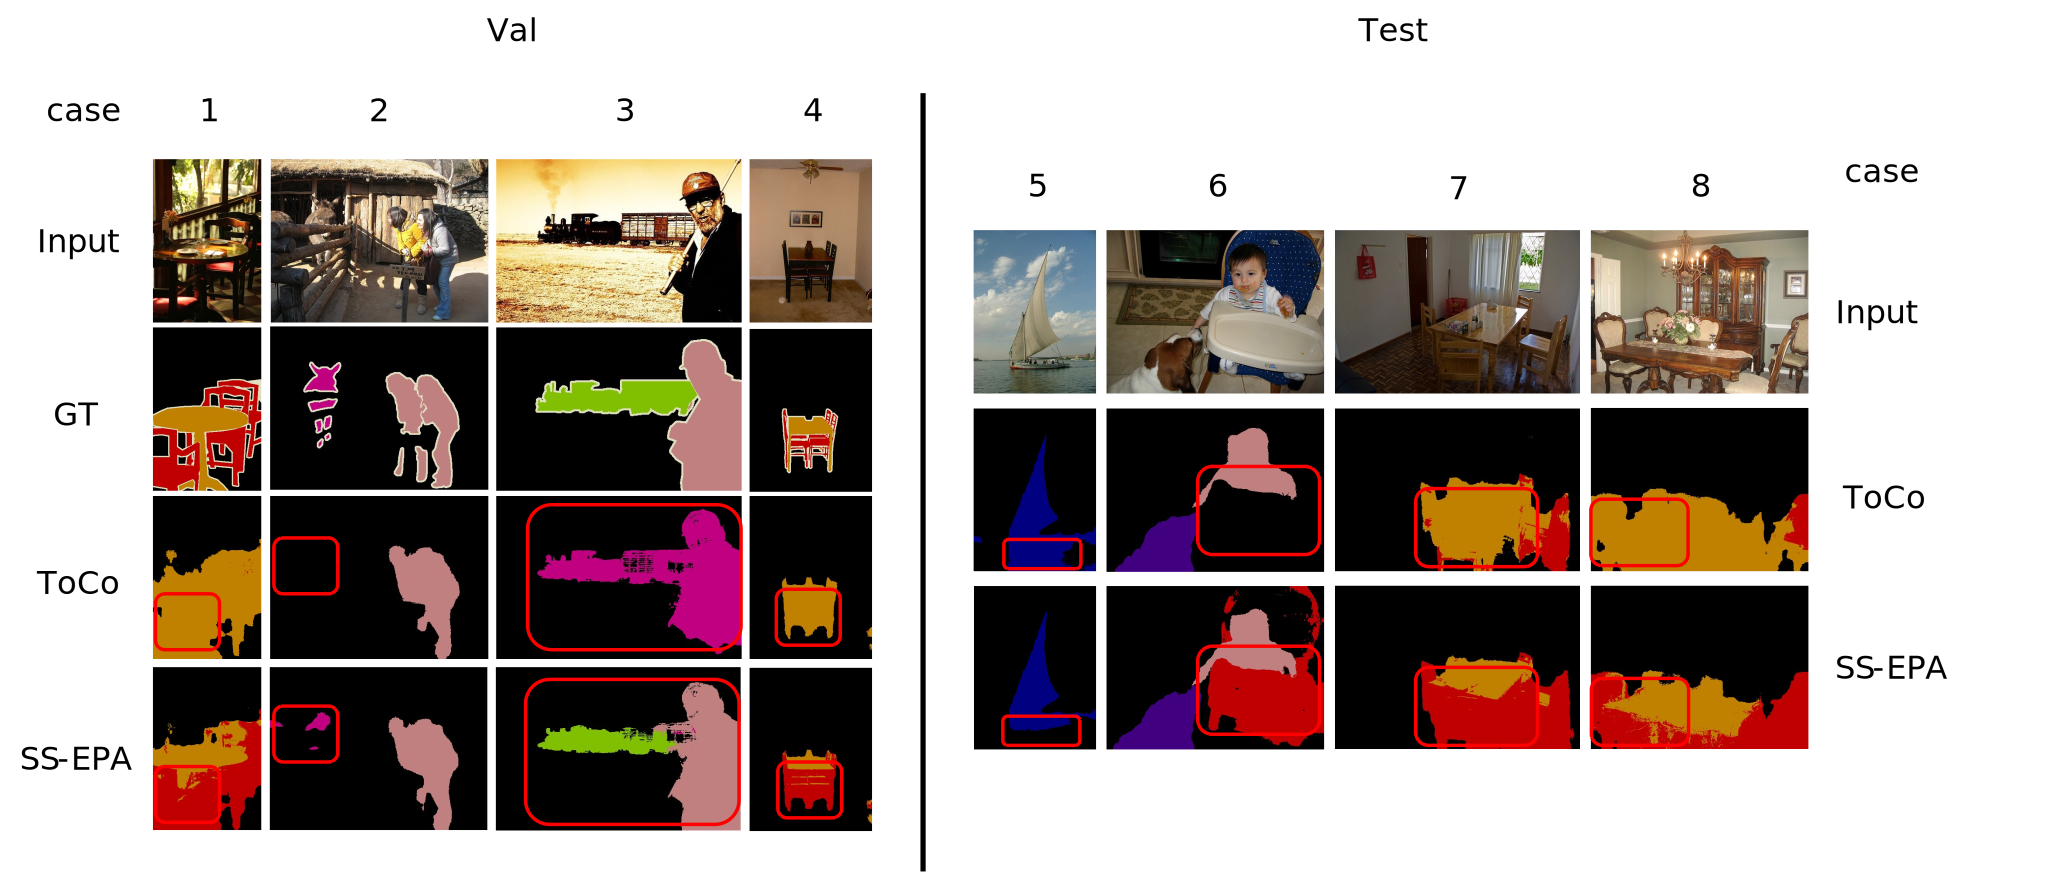
\includegraphics[width=6in]{fig/fig7_h.pdf}}
    \begin{CJK*}{UTF8}{fs}
        \caption{分割结果的可视化结果,左半部分为VOC验证集(Val),从上到下依次为输入图片(input),分割真值标签(GT),ToCo分割结果,SS-EPA分割结果。右半部分为VOC测试集(Test),从上到下依次为输入图片(input),ToCo分割结果,SS-EPA分割结果。红框部分为显著提升区域。}\label{fig7}
    \end{CJK*}
\end{figure*}


\vspace{2mm}

\begin{CJK*}{UTF8}{zhhei}
    \subsection{消融实验}
\end{CJK*}

% \begin{table*}[!htbp]
%     \small
%     \setlength{\tabcolsep}{6mm}
%     \centering
%     \caption{分割结果定量评估(单位mIoU\%)}\label{table3}
%     \begin{tabular}{lccc}
%         \toprule
%         Method & Pseudo label(train) & Seg(val) & Seg(test) \\
%         \midrule
%         ToCo & 77.3 & 71.1 & 72.21 \\
%         SS-EPA(w/o Patch Affinity) & 76.2 & 71.3 & 71.62 \\
%         SS-EPA(with Patch Affinity) & 79.0 & 71.9 & 72.73 \\
%         \textbf{SS-EPA(with Patch Affinity HAAF)} & \textbf{79.5} & \textbf{72.4} & \textbf{73.34} \\  
%         \bottomrule
%     \end{tabular}
% \end{table*}


\begin{CJK*}{UTF8}{zhhei}
    \subsubsection{补丁语义亲和力分析}
\end{CJK*}

表\ref{table3}呈现了关于伪标签和分割结果的消融实验定量评估。结果表明,使用不加HAAF增强的补丁语义亲和力后,SS-EPA可以生成更加优质的伪标签并提高分割性能。其中伪标签提升了2.8\%,分割性能在验证集和测试集上分别提升了0.6\%和1.1\%,分割的准确率更高。从图5可看出尽管在未使用HAAF的情况下存在噪声与错误,补丁语义亲和力仍有效优化了初始 CAM。

\begin{table}[!htbp]
    % \setlength{\tabcolsep}{6mm}
    \centering
    \caption{分割结果定量评估(单位mIoU\%)}\label{table3}
    \tiny
    \begin{tabular}{lccc}
        \toprule
        Method & Pseudo label(train) & Seg(val) & Seg(test) \\
        \midrule
        ToCo & 77.3 & 71.1 & 72.21 \\
        SS-EPA(w/o Patch Affinity) & 76.2 & 71.3 & 71.62 \\
        SS-EPA(with Patch Affinity) & 79.0 & 71.9 & 72.73 \\
        \textbf{SS-EPA(with Patch Affinity HAAF)} & \textbf{79.5} & \textbf{72.4} & \textbf{73.34} \\  
        \bottomrule
    \end{tabular}
\end{table}

\begin{CJK*}{UTF8}{zhhei}
    \subsubsection{HAAF分析}
\end{CJK*}

如\ref{section3.3_HAAF}节中所说,补丁语义亲和力存在噪声与错误,直接使用补丁语义亲和力并不合适。本文提出的HAAF模块显著减少了语义亲和力中的噪声和错误,并减少计算资源占用。从表3中可以看出,HAAF进一步提升了伪标签和分割结果的mIoU分数,其中伪标签提升了0.5\%,分割性能在验证集和测试集上分别提升了0.5\%和0.6\%。

\begin{table}[!htbp]
    % \setlength{\tabcolsep}{7mm}
    \centering
    \caption{SS-EPA计算资源占用实验结果评估(单位GB)}\label{table4}
    \tiny
    \begin{tabular}{lccc}
        \toprule
        Method & Backbone & Batchsize 1 & Batchsize 2 \\
        \midrule
        SS-EPA(w/o Patch Affinity) & ViT-B & 6.6 & 10.4 \\
        SS-EPA(with Patch Affinity) & ViT-B & 13.2 & 23.6 \\
        \textbf{SS-EPA(with Patch Affinity HAAF)} & \textbf{ViT-B} & \textbf{8.3} & \textbf{12.6} \\  
        \bottomrule
    \end{tabular}
\end{table}

表\ref{table4}展示了 SS-EPA 的计算资源占用评估,分别评估了 batchsize~1 和 batchsize~2 的实验结果。结果表明,在不使用 HAAF 的情况下,整个 SS-EPA 需要占据较高的的计算资源, batchsize 为 $1$ 时需要13.2GB显存, batchsize 为 $2$ 时则需要23.6GB。而 HAAF 可以将计算资源占用降低到 8.3GB 和 12.6GB ,显著减少了对计算资源的需求,提升了计算效率。

\begin{CJK*}{UTF8}{zhhei}
    \subsubsection{Backbone分析}
\end{CJK*}


表\ref{table5}展示了不同backbone下的SS-EPA和基线方法ToCo的实验结果评估。结果表明,SS-EPA在使用不同backbone的情况下比ToCo更好,在VOC验证集和测试集上的分割性能都更加优秀。其中表现最好的backbone是 vit-base-patch16-224 。与使用更高分辨率的 vit-base-patch16-384 相比,低分辨率的 vit-base-patch16-224 具有更好的泛化能力,不太容易过拟合到训练数据中的特定细节。而 vit-small-patch16-224 只有$8$层 Transformer 块,参数量和计算量都相对较少,导致其在捕捉图像中的复杂特征和细节时能力有限。

\begin{table*}[!htbp]
    \small
    \setlength{\tabcolsep}{6mm}
    \centering
    \caption{ SS-EPA不同Backbone实验结果评估(单位mIoU\%)}\label{table5}
    \begin{tabular}{lccccc}
        \toprule
        Method & Backbone & Depth & Img\_size & Seg(val) & Seg(test) \\
        \midrule
        ToCo & vit-small-patch16-224 & 8 & $224\times 224$ & 55.0 & 52.7 \\
        SS-EPA & vit-small-patch16-224 & 8 & $224\times 224$ & 57.6 & 50.2 \\
        ToCo & vit-base-patch16-384 & 12 & $384\times 384$ & 71.1 & 71.8 \\
        SS-EPA & vit-base-patch16-384 & 12 & $384\times 384$ & 71.7 & 71.9 \\
        ToCo & vit-base-patch16-224 & 12 & $224\times 224$ & 71.1 & 72.2 \\
        SS-EPA & vit-base-patch16-224 & 12 & $224\times 224$ & 72.4 & 73.3 \\    
        \bottomrule
    \end{tabular}
\end{table*}